\documentclass[xcolor=table, aspectratio=169]{beamer}

% !TEX engine = pdflatex
%\usepackage{arev}
\usepackage{amsmath,amssymb,amscd}
\usepackage{dsfont}
\usepackage{mathrsfs}
\usepackage{yfonts}
\usepackage{bm}
\usepackage{graphicx}
\usepackage{tabularx}
\usepackage{animate}
\usepackage{listings}
%\usepackage{mathtools}
%\usepackage{ifthen}
\lstset{language=GAP}

%\usepackage{xeCJK}
%\usepackage{fontspec}
%\newfontfamily\cjkfont{PingFang SC}
%\setCJKmainfont{PingFang SC}
\newcolumntype{x}{>{\centering\arraybackslash}X}
\renewcommand{\arraystretch}{1.5}
\newcommand{\uone}{\mathrm U(1)}
%\newcommand{\uone}{\mathbb R/\mathbb Z}
\DeclareMathOperator{\img}{img}
\DeclareMathOperator{\hhom}{Hom}
\DeclareMathOperator{\id}{id}
\usepackage{tikz}
	\usetikzlibrary{calc}
	\usetikzlibrary{arrows,shapes, positioning, matrix}
	\usetikzlibrary{decorations.markings}
	\tikzset{>=stealth}
	\tikzstyle arrowstyle=[scale=1]
	\tikzstyle directed=[postaction={decorate,decoration={markings,
 	   mark=at position .15 with {\arrow[arrowstyle]{stealth}}}}]
\tikzstyle string=[thick,postaction={decorate,decoration={markings,
    mark=at position .55 with {\arrow[arrowstyle]{stealth}}}}]
\tikzstyle dual_string=[dashed,postaction={decorate,decoration={markings,
    mark=at position .55 with {\arrow[arrowstyle]{stealth}}}}]

\tikzstyle dw=[thick,postaction={decorate,decoration={markings,
    mark=at position 1 with {\arrow[arrowstyle]{stealth}}}}]
\tikzstyle group=[mbg]
\newcommand*{\halfway}{0.5*\pgfdecoratedpathlength+.5*8pt}\tikzstyle arrowstyle=[scale=1]
\newcommand*{\halfwayb}{0.5*\pgfdecoratedpathlength}
\tikzstyle arrowstyle=[scale=1]
\tikzstyle fermion=[thick,postaction={decorate},decoration={markings,
    mark=at position \halfway with {\arrow[arrowstyle]{latex}}}]
\tikzstyle fermion2=[thick,postaction={decorate},decoration={markings,
        mark=at position \halfwayb with {\arrow[arrowstyle]{latex}}}]
\usepackage{tikz-cd}
\usepackage{pgffor}

\DeclareMathOperator{\tr}{Tr}
\DeclareMathOperator{\im}{Im}
\DeclareMathOperator{\re}{Re}

\mode<presentation>
{
  %\usetheme{Warsaw}
  % or ...
  %\useoutertheme{rectangle}
  \setbeamertemplate{frametitle}[default][center]
  \defbeamertemplate{itemize item}{flat}{\begin{pgfpicture}{-1ex}{0ex}{1ex}{2ex}
      \pgfpathcircle{\pgfpoint{0pt}{.6ex}}{0.6ex}
      \pgfusepath{fill}
    \end{pgfpicture}%
  }
  \defbeamertemplate{itemize subitem}{flat}{\footnotesize\raise0.5pt\hbox{\textbullet}}
  \defbeamertemplate{itemize subsubitem}{flat}{\footnotesize\raise0.5pt\hbox{\textbullet}}

  %\useinnertheme{circles}
  \setbeamertemplate{items}[flat]
  \setbeamertemplate{sections/subsections in toc}[circle]
  %\setbeamertemplate{blocks}[rounded]
  %\setbeamertemplate{title page}[default][colsep=-4bp,rounded=true]
  %\setbeamertemplate{part page}[default][colsep=-4bp,rounded=true]
	\setbeamertemplate{title page}[default][colsep=-4bp]
  \setbeamertemplate{part page}[default][colsep=-4bp]
  \setbeamercovered{transparent}
  %\usecolortheme{spruce}
  %\definecolor{THU}{RGB}{116,61,130}
  \definecolor{mbg}{RGB}{0,0,160}
  \setbeamercolor*{palette primary}{fg=white,bg=mbg}
  \setbeamercolor*{titlelike}{parent=palette primary}
  \setbeamercolor*{structure}{fg=mbg}
  \setbeamercolor{frametitle}{fg=white,bg=mbg}
  % or whatever (possibly just delete it)
  \setbeamercolor{block title}{bg=mbg,fg=white}
  \setbeamercolor{block body}{bg=mbg!15}


  \addtobeamertemplate{navigation symbols}{}{ \hspace{1em}%
    \usebeamerfont{footline}%
    \insertframenumber / \inserttotalframenumber }
}


%\usepackage[english]{babel}
% or whatever

%\usepackage[latin1]{inputenc}
% or whatever

%\usepackage{times}
%\usepackage[T1]{fontenc}
% Or whatever. Note that the encoding and the font should match. If T1
% does not look nice, try deleting the line with the fontenc.

\title[Intro to SptSet] % (optional, use only with long paper titles)
{SptSet: A GAP package for computing fermionic SPT classification and beyond}

\author[Y Qi] % (optional, use only with lots of authors)
{Yang~Qi}
% - Give the names in the same order as the appear in the paper.
% - Use the \inst{?} command only if the authors have different
%   affiliation.

\institute[Fudan] % (optional, but mostly needed)
{Department of Physics, Fudan University}
% - Use the \inst command only if there are several affiliations.
% - Keep it simple, no one is interested in your street address.

%\date{2016 Annual Meeting of Fudan CFTPP} % (optional, should be abbreviation of conference name)
%{Fudan University, Oct 13 2015}
%\date{Shenzhen Strongly Correlated Forum, Jan. 2020.}
\date{Croucher Summer Course at CUHK, 2023.}
% - Either use conference name or its abbreviation.
% - Not really informative to the audience, more for people (including
%   yourself) who are reading the slides online

\subject{Theoretical Physics}
% This is only inserted into the PDF information catalog. Can be left
% out.




% If you have a file called "university-logo-filename.xxx", where xxx
% is a graphic format that can be processed by latex or pdflatex,
% resp., then you can add a logo as follows:

\pgfdeclareimage[height=1cm]{university-logo}{../resources/fudan}
\logo{\pgfuseimage{university-logo}}

\AtBeginSection[]
{
  \begin{frame}<beamer>{Outline}
			\tableofcontents[currentsection,currentsubsection]
			%\begin{center}
			%	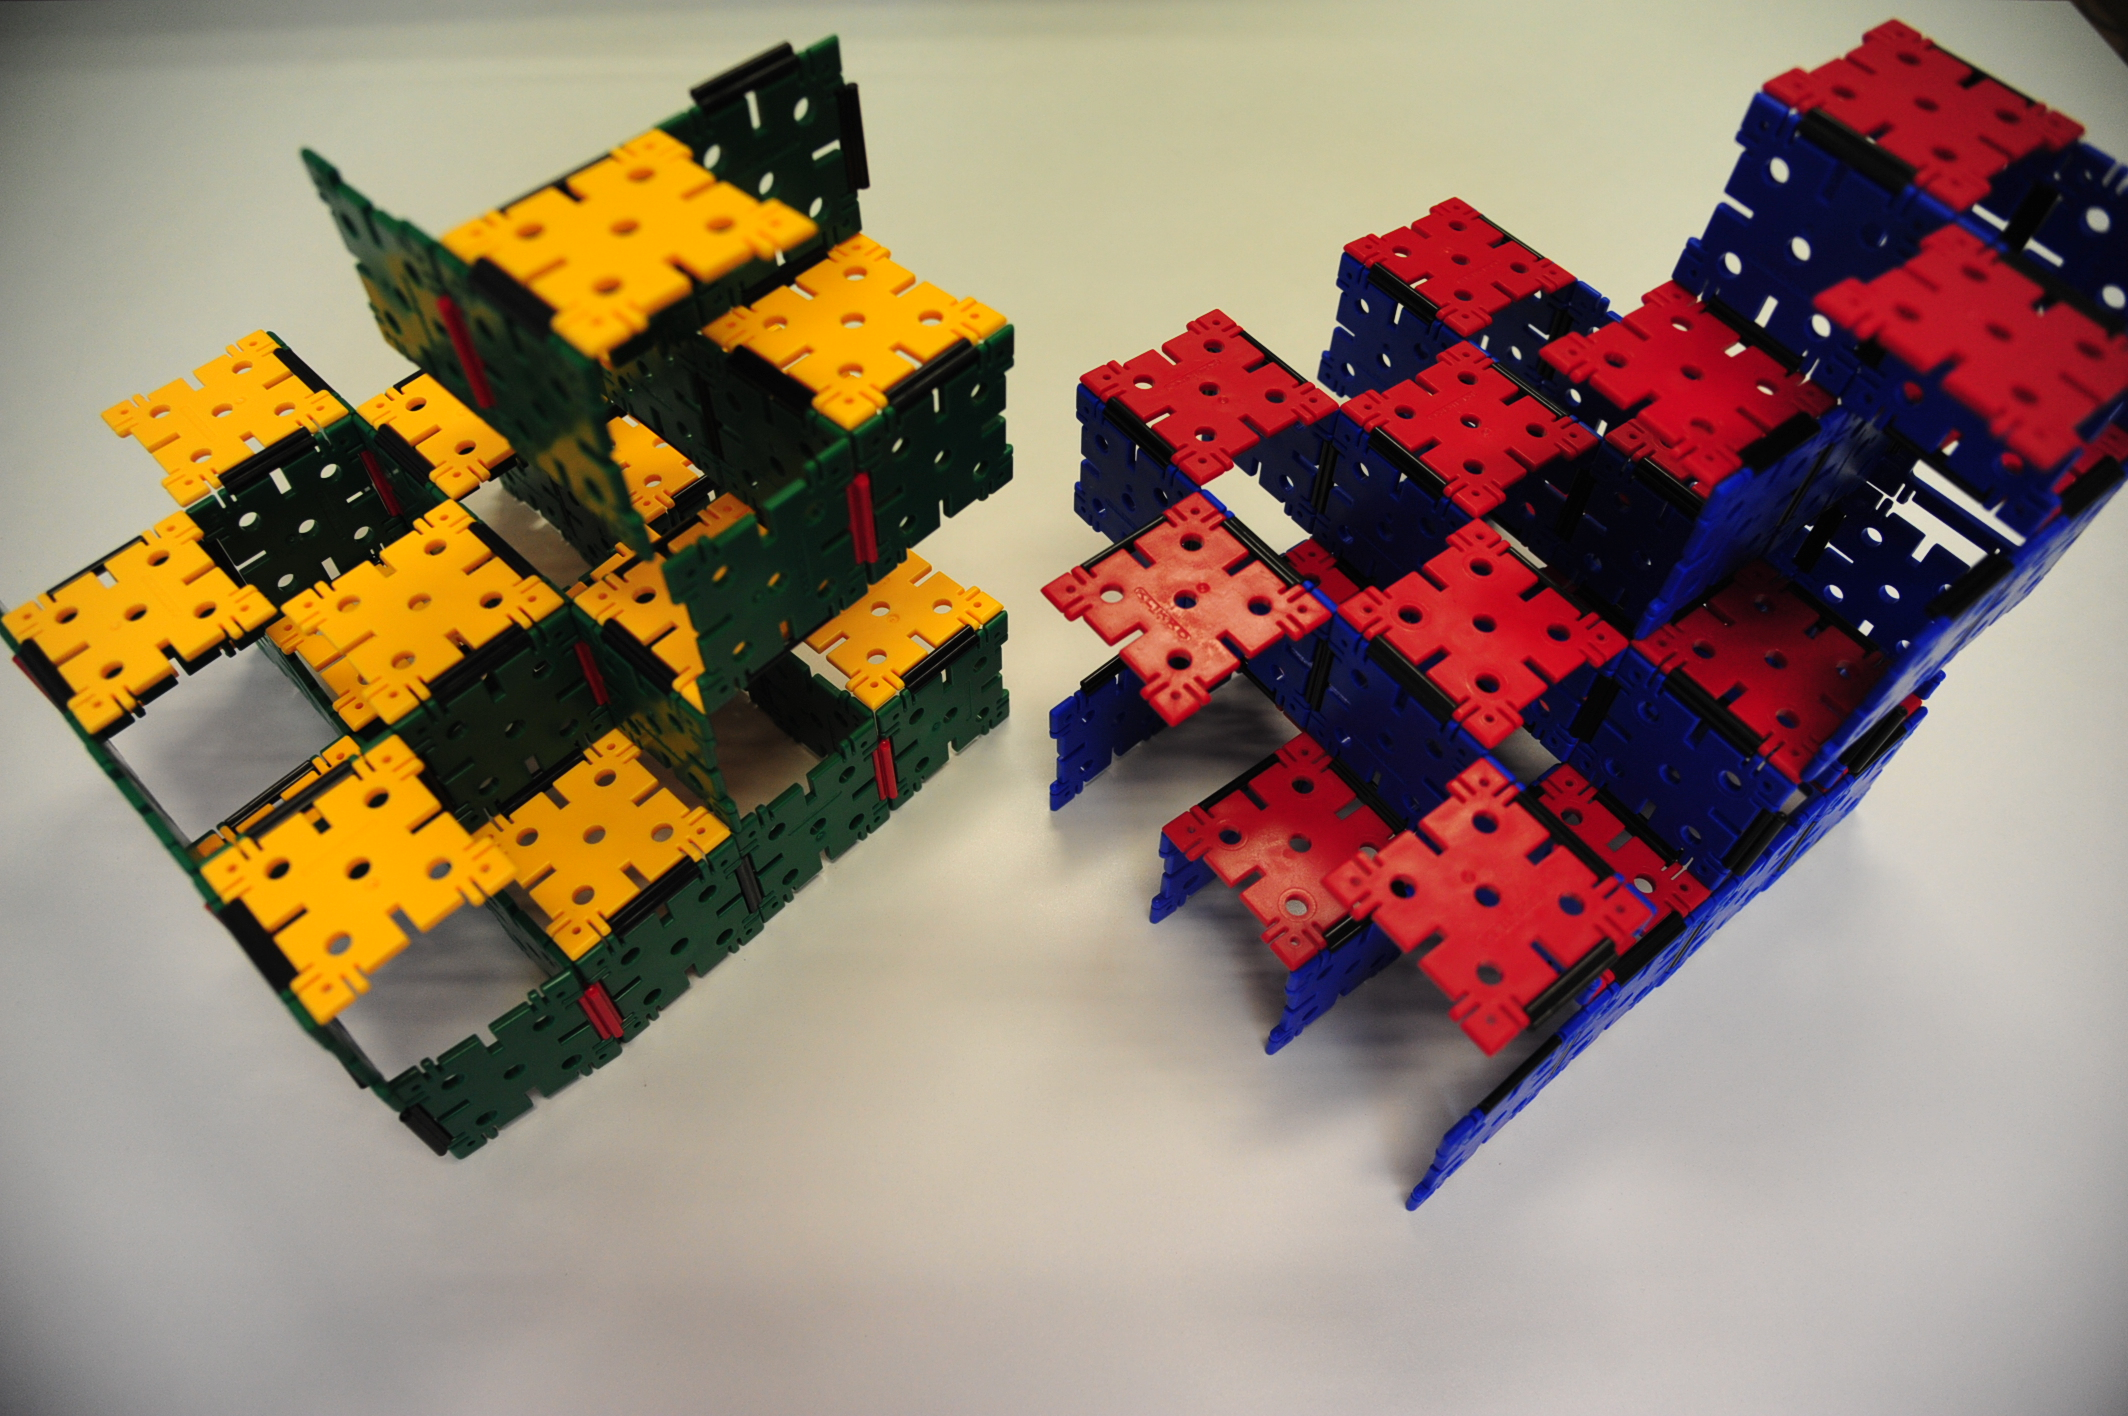
\includegraphics[height=4cm]{toys}
			%\end{center}
  \end{frame}
}


% Delete this, if you do not want the table of contents to pop up at
% the beginning of each subsection:

\begin{document}

\begin{frame}
  \titlepage
\end{frame}

\begin{frame}{Collaborators}
\begin{itemize}
%\item Yunqing Ouyang (欧阳云卿): Fudan University.
%\item Qing-Rui Wang (王晴睿): Chinese University of Hong Kong $\rightarrow$ Yale University.
%\item Zheng-Cheng Gu (顾正澄): Chinese University of Hong Kong.
\item Yunqing Ouyang: Fudan University $\rightarrow$ Huawei.
\item Qing-Rui Wang: YMSC, Tsinghua University.
\item Zheng-Cheng Gu: Chinese University of Hong Kong.
\begin{center}
	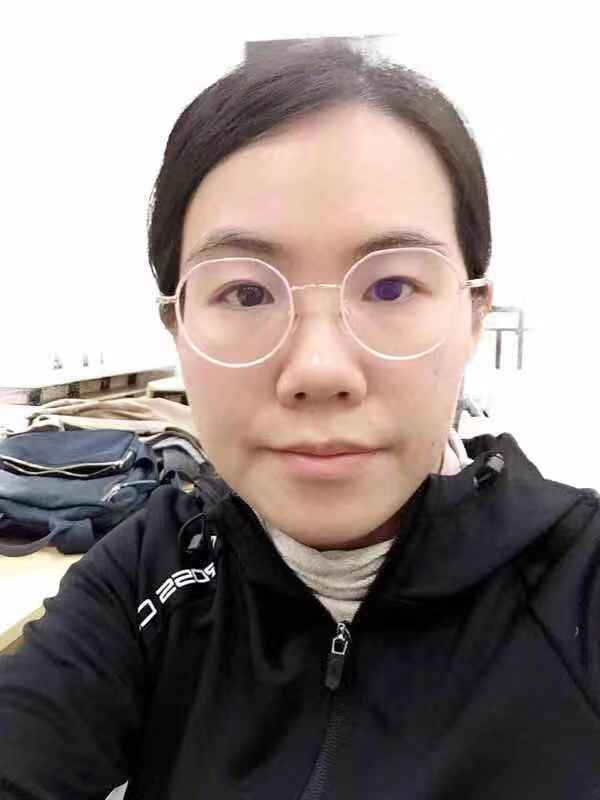
\includegraphics[height=3cm]{../people/yunqing}
	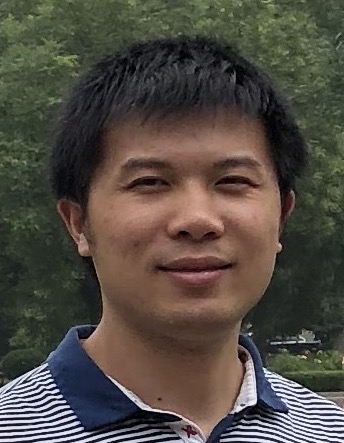
\includegraphics[height=3cm]{../people/qingrui}
	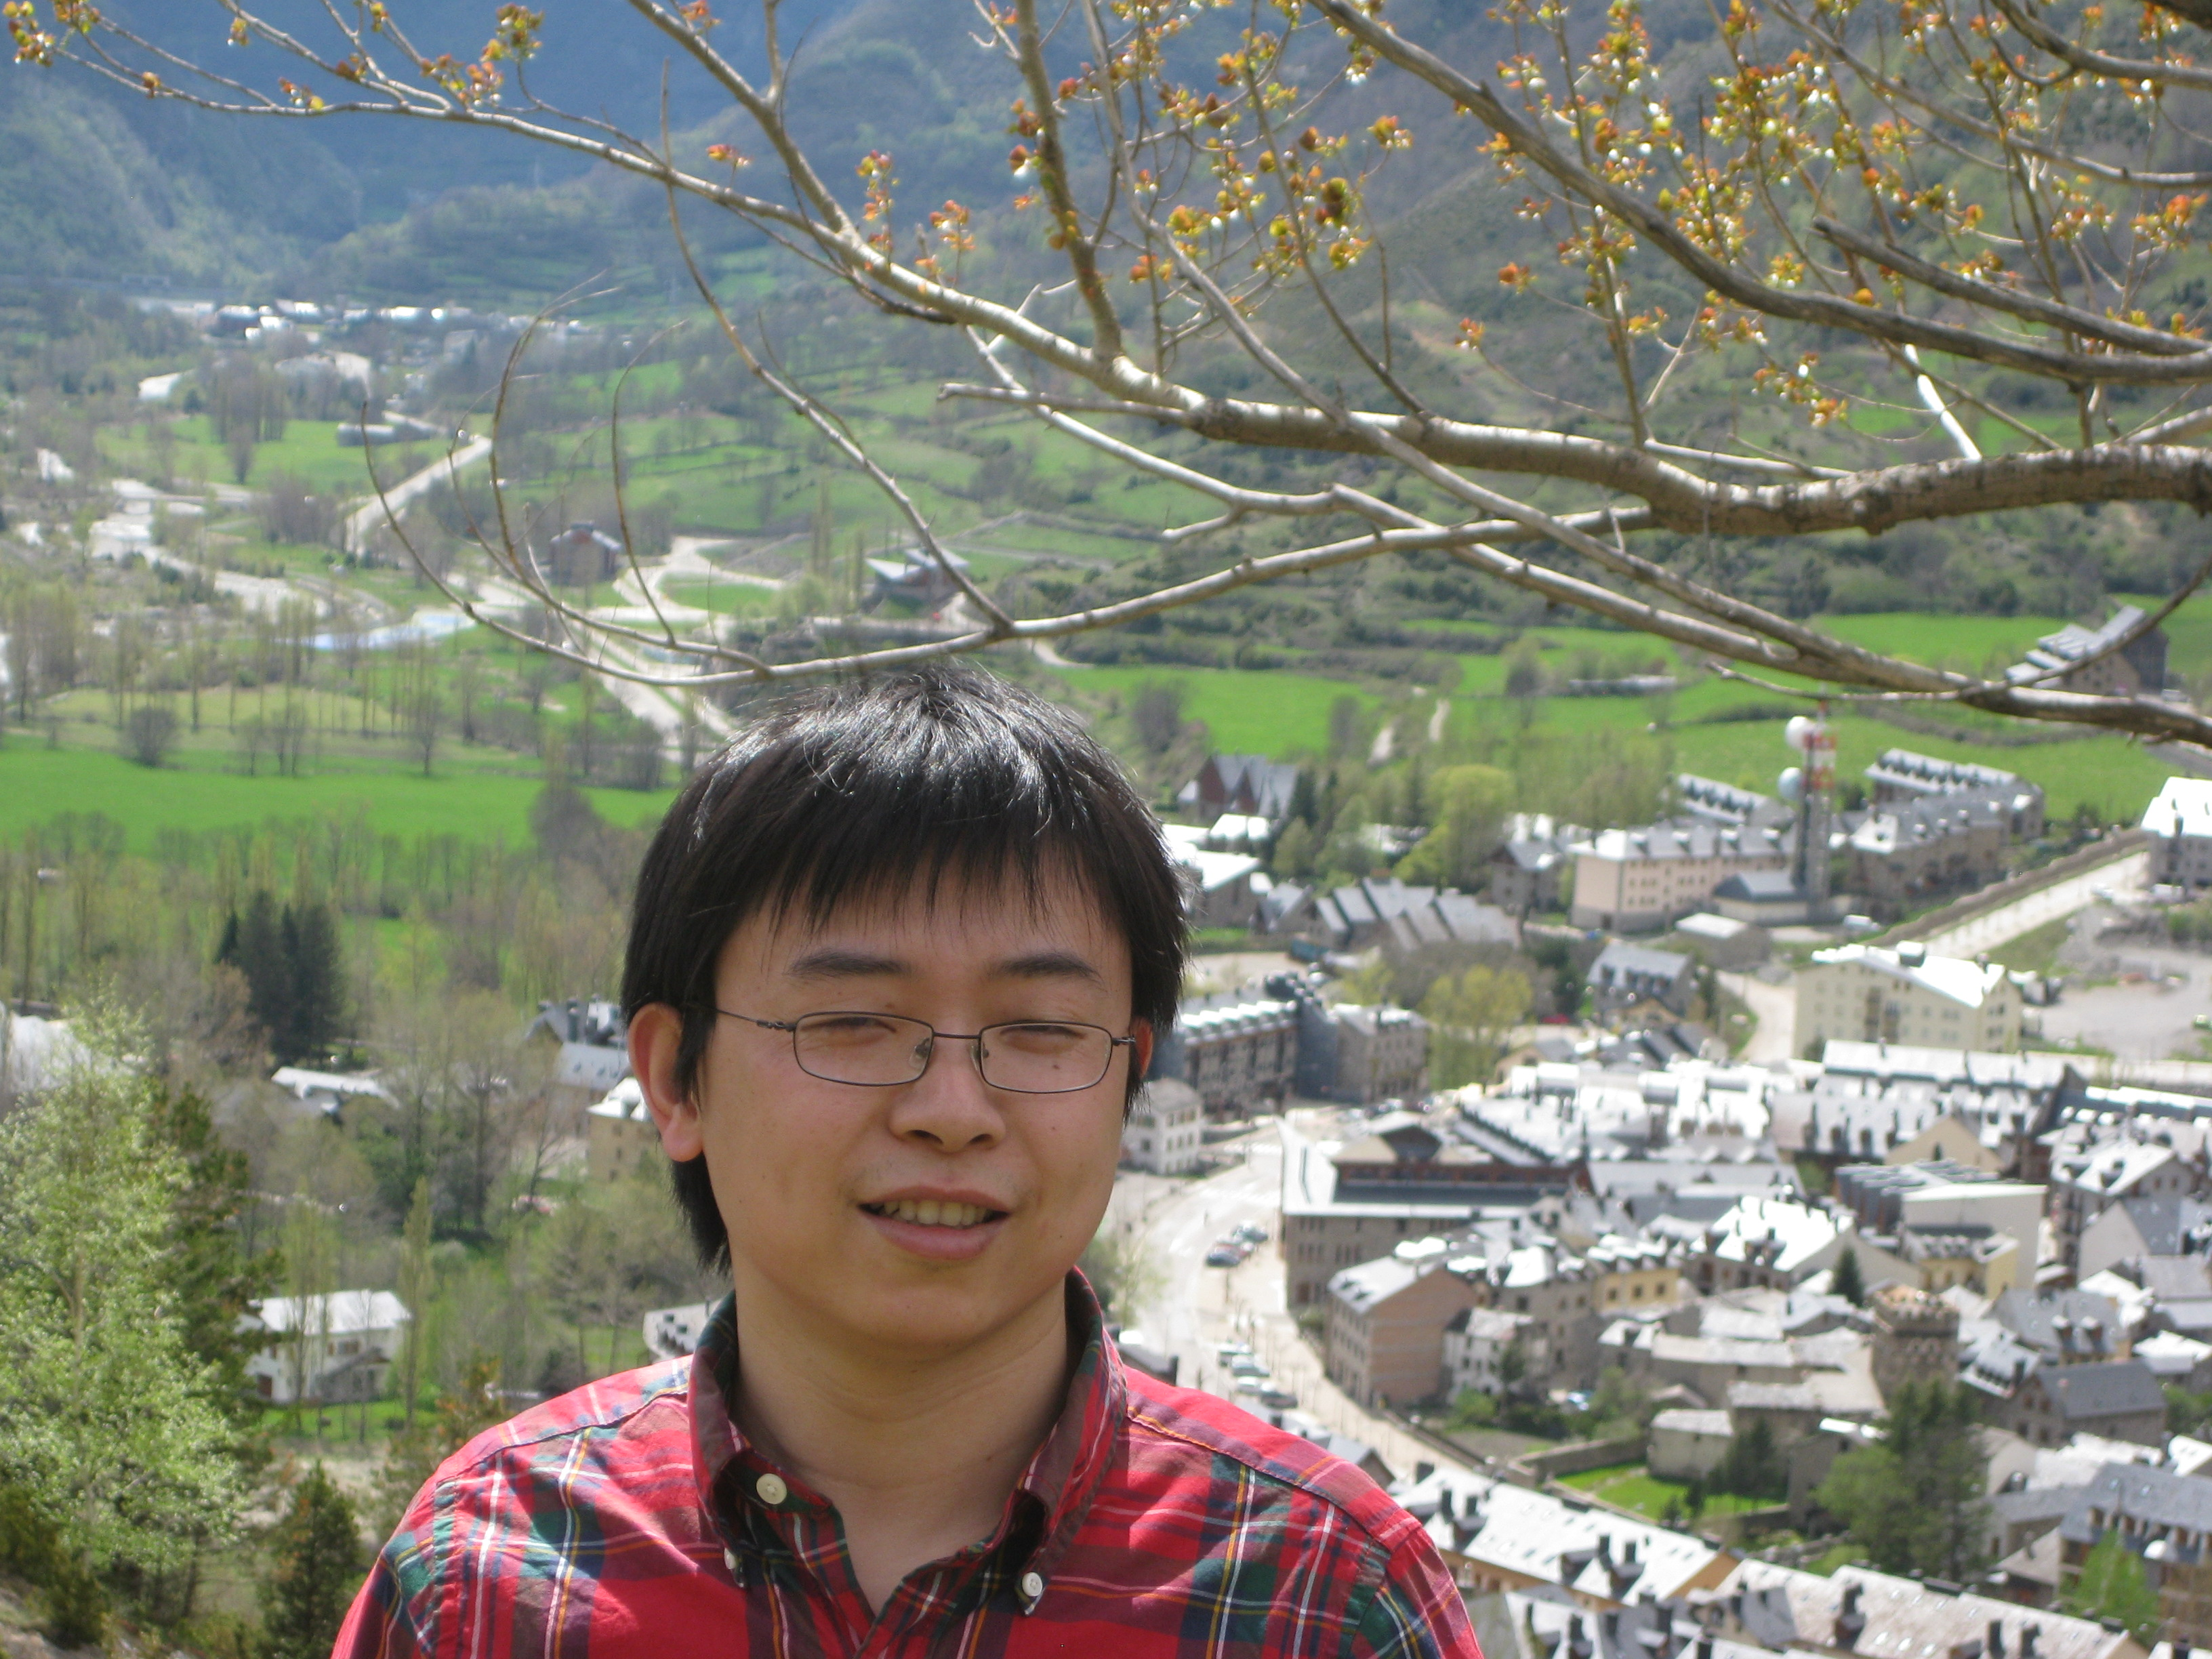
\includegraphics[height=3cm]{../people/zhengcheng}
\end{center}
\item Yunqing Ouyang, Qing-Rui Wang, Zheng-Cheng Gu and YQ,\\
Chin. Phys. Lett. \textbf{38}, 127101 (2021).
\item \url{https://github.com/yangqi137/SptSet}
\end{itemize}
\end{frame}

\section{Motivation: Why GAP?}

\begin{frame}
	\frametitle{The Problem: SPT and its classification}
	\begin{itemize}
		\item Symmetry-Protected Topological (SPT) States, examples: topological insulator (TI); Chern insulator, etc.
		\begin{center}
			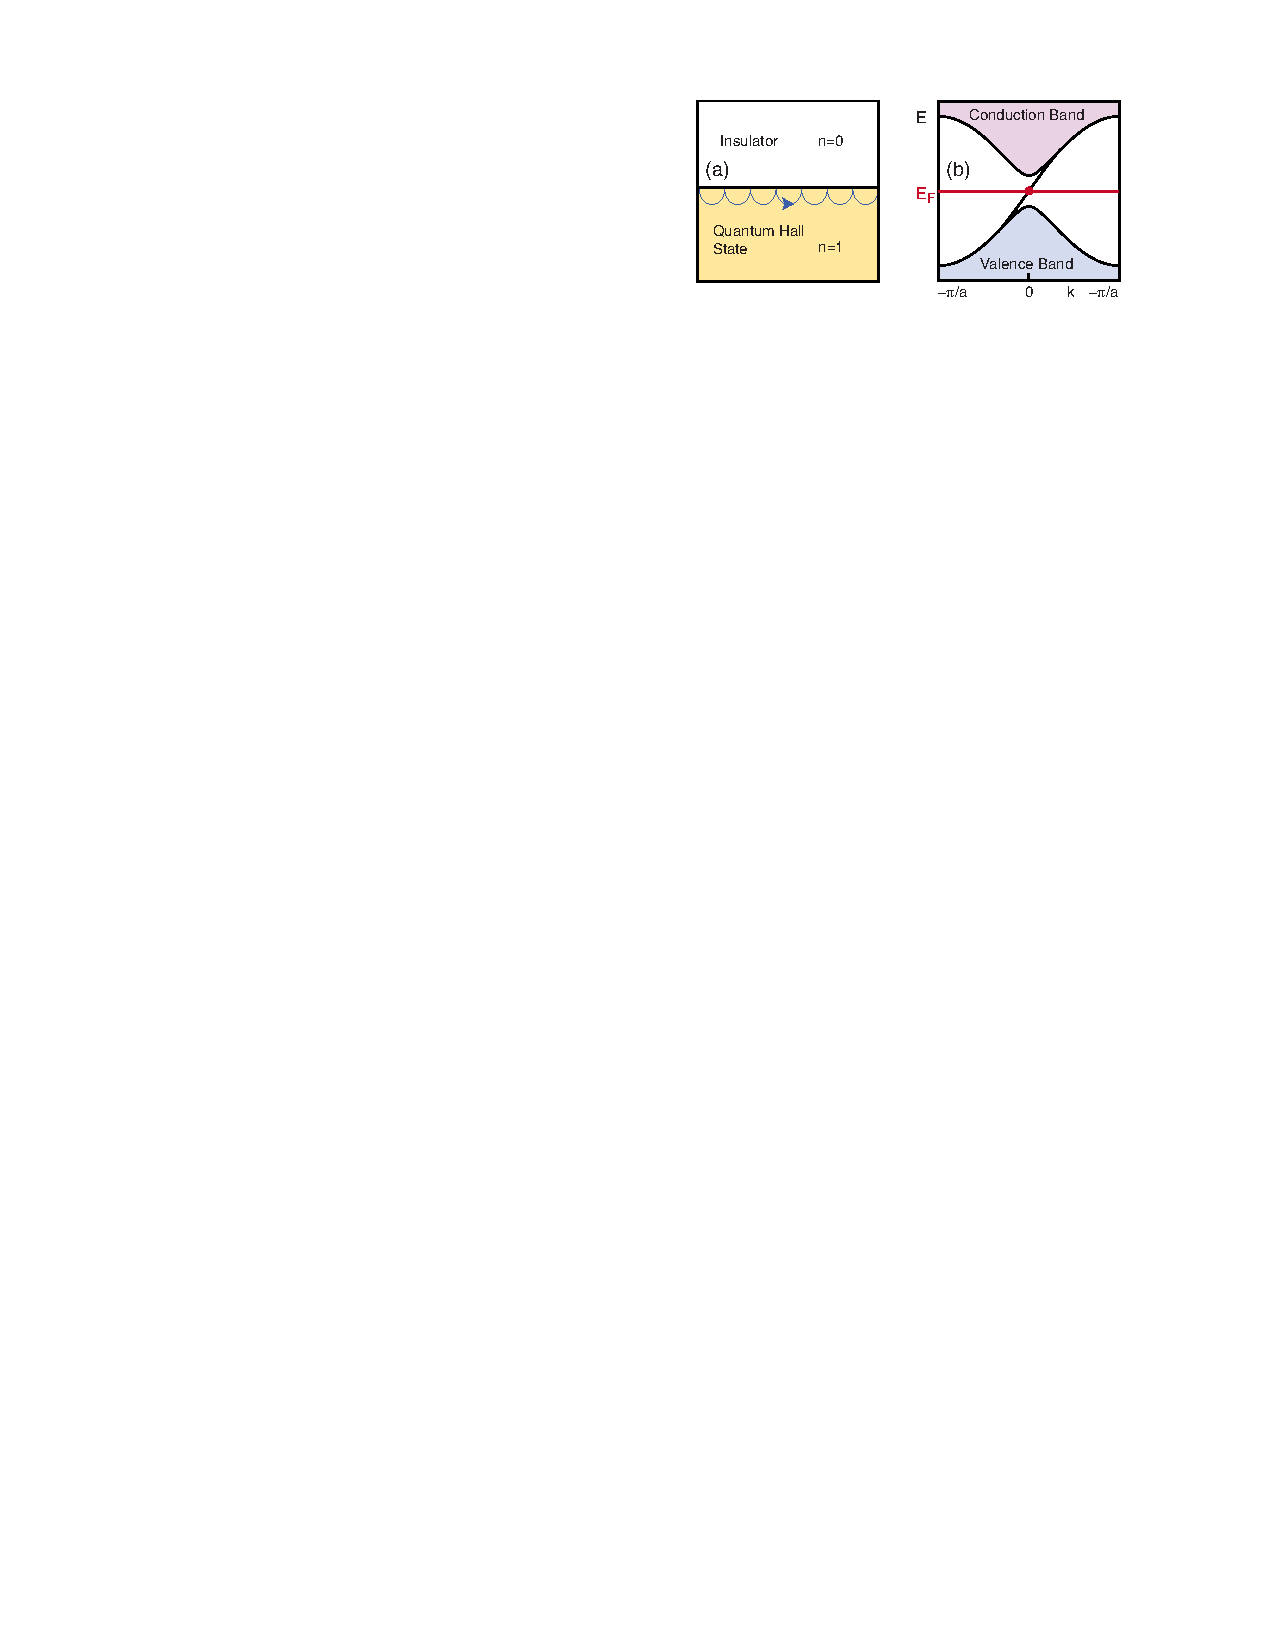
\includegraphics[width=6cm]{../spspt/qhe_edge}
		\end{center}
		{\small Classified by $\mathbb Z$: $[n]+[m]=[n+m]$; $[n]+[-n] = 0$.}	  
		\item SPT phases form an Abelian group under stacking.
		\item Classification is given by a generalized cohomology theory $\mathcal H^{d+1}(G)$,
		\begin{enumerate}
			\item Symmetry group $G$ (with more information...),
			\item Dimension $d$.
		\end{enumerate}
	\end{itemize}
\end{frame}

\begin{frame}[fragile]{Why GAP?}
  \begin{itemize}
  \item GAP = Group, Algorithm and Programming: \url{www.gap-system.org}.
  \item Advantage: easy to input a symmetry group.
    \begin{lstlisting}[basicstyle=\footnotesize]
      gap> G := CyclicGroup(4);
      pc group of size 4 with 2 generators>
      gap> G := DihedralGroup(6);
      pc group of size 4 with 2 generators>
      gap> G := SpaceGroup(3, 105);
      SpaceGroupOnRightBBNWZ( 3, 4, 5, 1, 2 )
    \end{lstlisting}
  \item Advantage: HAP package contains algorithms related to group-cohomology calculation.			
  \end{itemize}
\end{frame}

\section{Structure: fSPT and general invertible Topological Order classification}

\begin{frame}[fragile]
	\frametitle{Bosonic SPT: group cohomology and HAP}
	\begin{itemize}
		\item bSPT: classified by $H^{d+1}[G,\uone]$.
		\item $H^{d+1}[G,\uone]$ ``='' $H^{d+2}[G,\mathbb Z]$. \emph{See X-G Wen, PRB \textbf{91}, 205101 (2015)}
                \item Can be calculated using the HAP package in GAP.
	\end{itemize}
	\begin{columns}
		\column{.5\columnwidth}
	\begin{lstlisting}[basicstyle=\footnotesize]
gap> LoadPackage("HAP");
gap> G := CyclicGroup(4);
pc group of size 4 with 2 generators>
gap> GroupCohomology(G, 2);
[ 4 ]
gap> GroupCohomology(G, 3);
[  ]
gap> GroupCohomology(G, 4);
[ 4 ]
gap> GroupCohomology(G, 5);
[  ]
\end{lstlisting}
	\column{.5\columnwidth}
	\[H^{2n+1}[\mathbb Z_4,\uone] = \mathbb Z_4\]
	\[H^{2n}[\mathbb Z_4,\uone] = \mathbb Z_1\]
	\end{columns}
\end{frame}

\begin{frame}
  \frametitle{Fermionic SPT states}
  \begin{itemize}
  \item Atiyah–Hirzebruch Spectral Sequence for a generalized cohomology theory:
    \[E_2^{pq} = H^p(G, \mathcal H^q(*)) \Rightarrow \mathcal H^{p+q}(G).\]
    \begin{itemize}
    \item $\mathcal H^q(*)$: $q$-dimensional invertible topological order (iTO).
    \[\Omega^0=\uone_T,\quad\Omega^1=\mathbb Z_2,\quad\Omega^2=\mathbb Z_2,\quad\Omega^3=\mathbb Z_T.\]
    \item Physical interpretation: Decorate codim-$p$ DW w/ $(q+1)$-d iTOs.
    \end{itemize}
  \item Wave function: $\psi\in \Psi^d(G)$: $\psi=\begin{pmatrix}\psi^0&\psi^1&\cdots&\psi^{d+1}\end{pmatrix}$.
  \end{itemize}
  \begin{center}
    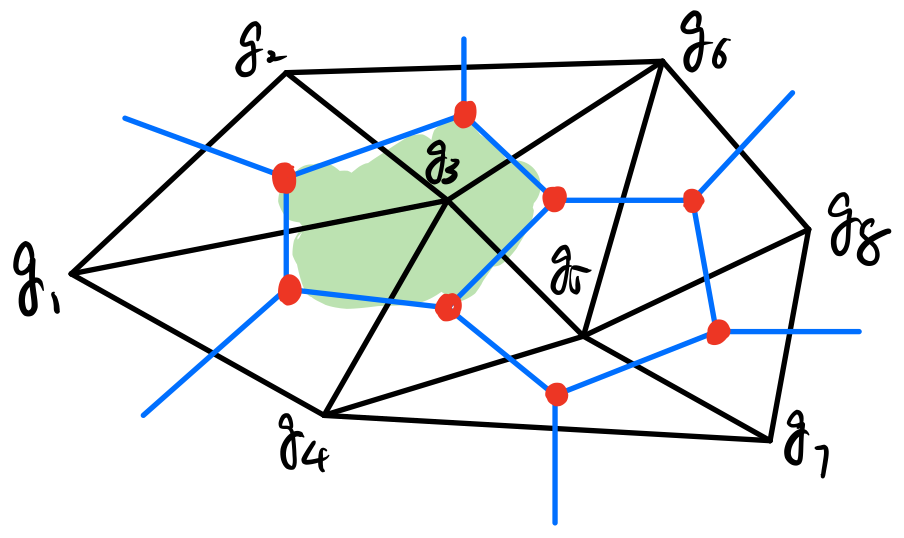
\includegraphics[height=3cm]{decoration}
  \end{center}
\end{frame}

\begin{frame}
  \frametitle{Symmetry group: $G$, $s$ and $\omega_2$}
  Symmetry is specified by three pieces of information:
    \begin{enumerate}
    \item (Bosonic) symmetry group $G$;
    \item Unitary/antiunitary structure: $s:G\rightarrow \mathbb Z_2$; Example: s(T)=1.
    \item $\omega_2\in H^2(G, \mathbb Z_2^f)$, classifying $1\rightarrow\mathbb Z_2^f\rightarrow G_f\rightarrow G\rightarrow1$. Example: $\omega_2(T, T)=\pm1$.
    \end{enumerate}
	$\mathcal H^{d+1}(G)$ depends on $(G, s, \omega_2)$.
\end{frame}

\begin{frame}
	\frametitle{Coboundary operation}
	\begin{itemize}
		\item Consider the coboundary of a single-layer state
		$\psi = \begin{pmatrix}0&\cdots&\psi^p&\cdots&0\end{pmatrix}$.
		\item $\delta\psi$ only contains layers $p'<p$:
		$\delta\psi=\begin{pmatrix}0&\cdots&d\psi^p&(\delta\psi)^{p+2}\cdots&(\delta\psi)^{d+2}\end{pmatrix}$.
		\item We denote $(\delta\psi)^{p'}=\mathcal D^{p, d-p+1}_{p'-p}(\psi^p)$.
		$D^{pq}_r:C^p(G_b,\Omega^q)\rightarrow C^{p+r}(G_b,\Omega^{q-r+1})$.
		\item $d$ is like an upper-triangular matrix.
		\item Examples: in 2d, $G=G_b\times\mathbb Z_2^f$
		\begin{align*}
			\mathcal D_2^{12} &= s\cup\psi^1\cup\psi^1,\\
		  \mathcal D_2^{21} &= \frac12\psi^2\cup\psi^2
		  +\frac12\psi^2\cup_1d\psi^2
		  +\mathcal O_4'(d\psi^2).
		\end{align*}
		\[  O_4'(\psi^2)(01234)
		  =\frac12d\psi^2(0124)d\psi^2(0234)
		  -\frac14\{d\psi^2(0123)[1-d\psi^2(0124)] \mod 2\}.\]
	\end{itemize}
\end{frame}

\begin{frame}
	\frametitle{Stacking operation}
	\begin{itemize}
		\item Not a simple component-wise addition:
		$\psi_1\boxplus\psi_2\neq (\psi_1^{d+1}+\psi_2^{d+1},\ldots,\psi_1^0+\psi_2^0)$.
		\item Reason: reordering of fermionic degrees of freedom.
		\item Result on the $p$-th layer will be twisted by higher layers.
		\[(\psi_1\boxplus\psi_2)^p = \psi_1^p + \psi_2^p
    + \mathcal A^{p,d-p+1}(\psi_1^{d+1},\psi_2^{d+1},\ldots,\psi_1^{p+1}, \psi_2^{p+1}),\]
		\item Examples: in 2d, $G=G_b\times\mathbb Z_2^f$
		\begin{align*}
		  \mathcal A^{21} &= \psi^1_1\cup\psi^1_2;\\
		  \mathcal A^{30} &= \frac12\psi^2_1\cup_1\psi^2_2 + \frac12 (\psi^1_1\cup\psi^1_2)\cup_1(\psi^2_1+\psi^2_2).
		\end{align*}
	\end{itemize}
	\begin{center}
		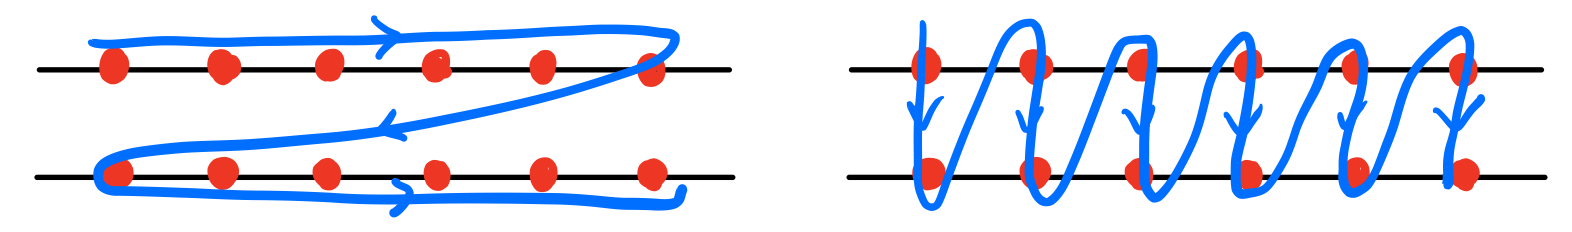
\includegraphics[height=2cm]{forder}
	\end{center}
\end{frame}

\begin{frame}[fragile]
	\frametitle{Input formulas into the SptSet package}
	\begin{itemize}
		\item The functions $\mathcal A^{pq}$ and $\mathcal D^{pq}_r$ needs to be inputed.
		\item Example: $\mathcal D_2^{12} = s\cup\psi^1\cup\psi^1$.
	\end{itemize}

	\begin{block}{GAP realization}
	\begin{lstlisting}[basicstyle=\footnotesize]
	SptSetInstallCoboundary(ss, 2, 1, 2,
	function(n1, dn1)
		return {g1, g2, g3} -> (s(g1) * n1(g2) * n1(g3));
	end);
	\end{lstlisting}
	\end{block}

\end{frame}

\begin{frame}[fragile]
	\frametitle{SptSet: computing fSPT and beyond}
	Consider 2D fSPT, $G_f=\mathbb Z_4\times\mathbb Z_2^f$:
\begin{lstlisting}[basicstyle=\footnotesize]
gap> LoadPackage("SptSet");;
gap> G := CyclicGroup(4);;
gap> R := ResolutionFiniteGroup(G, 6);;
gap> utAct := SptSetTrivialGroupAction(G);;
gap> ss := FermionEZSPTSpecSeq(R, utAct);;
gap> FermionSPTLayers(ss, 2);
[ <ZL-Module with torsions [ 2 ]>, <ZL-Module with torsions [ 2 ]>,
  <ZL-Module with torsions [ 4 ]> ]
gap> z2tAct := GroupHomomorphismByImagesNC(G, GL(1, Integers),
>   GeneratorsOfGroup(G), [ [[-1]], [[1]] ]);;
gap> ss := FermionEZSPTSpecSeq(R, z2tAct);;
gap> FermionSPTLayers(ss, 2);
[ <ZL-Module with torsions [ 2 ]>, <ZL-Module []>, <ZL-Module []> ]
\end{lstlisting}

\end{frame}

\begin{frame}[fragile]
  \frametitle{Example: fSPT for 2D wallpaper groups}
  \begin{itemize}
  \item Crystalline equivalence principle (Thorngren \& Else, PRX 2018):
  \begin{enumerate}
	\item Calculate the equivalent problem: $G$ is treated as an \alert{onsite} symmetry group;
	\item Inproper operation $\Rightarrow$ antiunitary: $s(g) = \det g$;
	\item Spin-$\frac12$ $\Leftrightarrow$ spinless.
	\[\omega_2 = \omega_2' + \omega_2^{s=1/2}.\]
  \end{enumerate}
  \item Results consistent w/ real-space construction (Jian-Hao Zhang, et al).
  \item Battery included in \lstinline|SptSet|: construction of $\omega_2^{s=1/2}$ for 2d and 3d space groups
  \begin{lstlisting}[basicstyle=\footnotesize]
	w2 := Spin12Factor(d, it);
  \end{lstlisting}
\end{itemize}
\end{frame}

\begin{frame}[fragile]{Example: fSPT for 2D wallpaper groups}
	\url{SptSet/examples/fspt_2d_s12.g}
	\begin{lstlisting}[basicstyle=\footnotesize]
    for it in [2..17] do
      SG := SpaceGroupBBNWZ(2, it);
      fSG := IsomorphismPcpGroup(SG);
      SG1 := Image(fSG);
      R := ResolutionAlmostCrystalGroup(SG1, 6);
      gs := GeneratorsOfGroup(SG);
      w := Spin12Factor(2, it);
      ww := {g1, g2} -> w(PreImageElm(fSG, g1), PreImageElm(fSG, g2));
      f := GroupHomomorphismByImagesNC(SG1, GL(1, Integers),
        List(gs, x -> Image(fSG, x)),
        List(gs, x -> [[DeterminantMat(x)]]));

      SS := FermionSPTSpecSeq(R, f, ww);
      FermionSPTLayersVerbose(SS, 2);
    od;
  \end{lstlisting}
\end{frame}

\section{Algorithm: simplified resolution and chain maps}

\begin{frame}
  \frametitle{Simplified resolution and chain maps}
  \begin{itemize}
  \item A problem: cochains $\alpha(g_0,\ldots,g_n)$ are too complicated to deal with.
    \begin{itemize}
    \item View cochain space as a ``linear space'': $N_n = (|G|-1)^n$;
    \item Solving the cocycle equations: $O(N_n^3)\sim O((|G|-1)^{3n})$.
    \item Impossible for infinite groups (such as the space groups).
    \end{itemize}
  \item Solution: A simplified resolution: a simplified basis replacing $[g_0,\ldots,g_n]$.
    \begin{itemize}
    \item Simple models of $BG$.
    \item $\mathbb Z:$ $N_n=0$ for $n>1$; $\mathbb Z_n$: $N_n=1$.
    \item $1\rightarrow N\rightarrow G\rightarrow Q\rightarrow1$: $N_n^G=\sum_{p+q=n}N_p^NN_q^Q.$ (a ``twisted'' tensor product).
    \end{itemize}
  \item Chain maps: a ``compiler'' converting formulas from the standard basis to the simplified basis.
  \item Allows computation for infinite (discrete) groups.
  \end{itemize}
\end{frame}

\section{Summary and Outlooks}

\begin{frame}{Current status for fSPTs}
	\begin{itemize}
		\item 2d SPT states: Majorana + Complex fermion + Bosonic layers.
		\item Example: 17 wallpaper groups in ~5 minutes.
		\item Stacking rules are missing (work in progress with Xing-Yu Ren, Qing-Rui Wang and Zheng-Cheng Gu).
		\item 3d SPT states: one obstruction function is missing (work in progress with Shang-Qiang Ning and Zheng-Cheng Gu).
		\item Will be updated on \url{https://github.com/yangqi137/SptSet}.
	\end{itemize}
\end{frame}

\begin{frame}{Other tasks}
	\begin{enumerate}
		\item TIs: interacting fSPT with U(1) symmetry.
		\begin{itemize}
			\item Given $1\rightarrow U(1)_f\rightarrow G_f\rightarrow G\rightarrow 1$, we have
			\[E_2^{pq}=H^p(G, \mathcal H^q(U(1)))\Rightarrow \mathcal H^{p+q}(G_f).\]
			\item Jian-Hao Zhang, et al, PRResearch \textbf{4}, 033081 (2022).
			\item Can be computed using the \lstinline|InsulatorSPTSpecSeq| function.
		\end{itemize}

		\item ASPTs:
		\begin{itemize}
			\item $G_b$ is averaged symmetry, $\mathbb Z_2^f$ is exact.
			\item Remove the bSPT layer: $\mathcal H^0_A(*)=0$ in $E_2^{pq}=H^p(G_b, \mathcal H^q_A(*))$.
			\item Can be computed using the \lstinline|AvgFermionSPTSpecSeq| function.
		\end{itemize}
	\end{enumerate}
\end{frame}

\end{document}
